\section{Policy substrate and training provenance}
\label{s:substrate}
The rescue experiment freezes the complete endpoint. This section documents its construction for reproducibility; the assistance result does not identify a benefit of the conditioning branch.

\paragraph{Lineage and observations.}
Let $\theta_0$ be the released Xiaomi-Robotics-1-RoboCasa365 model. Rank-16, alpha-16 Action LoRA parameters $\alpha$ produce the adapted teacher $\theta_A=(\theta_0,\alpha)$. Only branch parameters $\phi$ are updated in the final training stage. The release alias A2000 refers to an unchanged adapter actually trained for 1,613 updates; B2000 records the branch endpoint at 2,000 updates. These names do not denote separately pretrained foundation models.

For each sample, the frozen visual-language pass returns $H\in\mathbb R^{S\times D}$, $D=2560$. Three cameras each supply four observed frames. The processor forms two temporal patch groups; the branch averages spatial tokens in the most recent group for each camera to obtain $\bar h_1,\bar h_2,\bar h_3$. Let $h_{\mathrm{last}}$ be the last valid post-video token in the released prompt order. The padded state history is $s\in\mathbb R^{4\times 60}$; only coordinates $0$--$13$ are valid, and the remaining coordinates are checked to be zero. The detached branch input and outputs are
\begin{align}
x&=[\bar h_1;\bar h_2;\bar h_3;h_{\mathrm{last}};
       \operatorname{vec}(s_{:,0:14})]\in\mathbb R^{4 D+56},\label{s:eq:input}\\
z&=\operatorname{SiLU}(W_e x+b_e)\in\mathbb R^{256},\qquad
\ell=W_s z+b_s\in\mathbb R^7,\\
\Delta_\phi&=\operatorname{reshape}(W_\Delta z+b_\Delta,6,1024).
\end{align}
The output projection $W_\Delta,b_\Delta$ is initialized to zero. Including the auxiliary stage head, the branch contains 4,216,839 trainable parameters. A scoped forward hook adds the residual to the native time-projector output before its six-channel reshape:
\begin{equation}
\widetilde m(t,o,s)=m_{\theta_A}(t)+\Delta_\phi(o,s).
\end{equation}
The native action transformer consumes this conditioning through adaptive normalization. The residual modifies conditioning, not a motor command. One visual-language pass serves each action query, and the same observation-derived residual is available to the five Euler evaluations. The hook is removed on normal and exceptional exits; reentrant requests are rejected.

\paragraph{Losses and information boundary.}
For demonstrated action chunk $a$, noise $\epsilon$, and flow time $t$, training uses $a_t=(1-t)\epsilon+ta$ and target $a-\epsilon$. Let $M_i$ combine valid action coordinates and time steps, with a nonempty mask for every sample. Define
\begin{equation}
\operatorname{MSE}_{M_i}(r)=\frac{\sum_jM_{ij}r_{ij}^2}{\sum_jM_{ij}}.
\end{equation}
Writing $v_{B,i}=v_{\theta_A,\phi}(a_{t,i},t_i\mid o_i,s_i)$ and $v_{A,i}$ for the frozen adapted teacher under the same inputs, the recorded objective is
\begin{align}
L_{\mathrm{flow}}&=\frac 1 B\sum_i\operatorname{MSE}_{M_i}\bigl(v_{B,i}-(a_i-\epsilon_i)\bigr),\\
L_{\mathrm{ret}}&=\frac 1 B\sum_i\operatorname{MSE}_{M_i}\bigl(v_{B,i}-\operatorname{stopgrad}(v_{A,i})\bigr),\\
L_{\mathrm{stage}}&=\frac 1 B\sum_i\mathbf 1[y_i\geq 0,\ q_i\geq 1]\operatorname{CE}(\ell_i,y_i),\\
L&=L_{\mathrm{flow}}+L_{\mathrm{ret}}+0.05 L_{\mathrm{stage}}.
\end{align}
The teacher retains its enabled LoRA and shares the student's noisy action, time, state embeddings, and cached visual-language context. Its evaluation uses no gradients and is checked not to mutate shared inputs or consume extra random state. Annotation confidence $q_i$ is detached; missing or low-confidence labels suppress only the auxiliary term. That term is normalized by all batch windows, not by admitted labels. Stage labels, stage confidence, and externally supplied stage residuals are excluded at inference. The seven logits do not select a hard option. Teacher consistency on training samples is a penalty, not a guarantee against rollout regressions.

\paragraph{Data and optimization.}
A2000 processed 80,000 sampled windows across 1,613 updates with changing batch size. B2000 processed 256,000 sampled windows across 2,000 updates at global batch size 128, learning rate $10^{-4}$, and gradient-clipping threshold 1.0; recorded elapsed training time was 8,453.98 s. These window counts can contain repeated samples and must not be described as distinct trajectories. Branch master parameters use FP32; the original model path retains recorded mixed precision. No unverified optimizer setting is inferred from the endpoint.

B samples Human300 replay and a 200-trajectory development collection in equal proportions. The collection covers 16 Composite-Seen tasks, with 168 training and 32 diagnostic held-out trajectories. Existing annotation fields supply stage targets; this stage adds neither new human labels, reasoning-model annotations, nor MimicGen data. The local sample-plan audit covers all 80,000 A entries and 256,000 B entries, marked as human data. Their task names lie within Human300 and do not intersect the 16 official Composite-Unseen tasks. This is an audit of the bound adaptation plans, not an independent reconstruction of the base model's pretraining data. The diagnostic trajectory split is not an unseen-task test. No further training is performed for language assistance.

\section{Evaluation manifest and execution record}
\label{s:execution}
The historical manifest has 18 Atomic-Seen, 16 Composite-Seen, and 16 Composite-Unseen tasks in pretraining scenes, each with 50 episodes. Policy and environment seeds are fixed in the range 2090900000--2090902499; registered task horizons are retained. Inference uses five Euler steps, replanning every 16 environment steps, history length four, observation interval two, and crop ratio 0.95. Original Counter reset source is checked before and after each episode. All 2,500 original episodes terminate with known outcomes: 1,496 successes and 1,004 failures, with no unattempted or infrastructure-unknown cases. Every original failure reaches its horizon. Equal episode allocation makes the task macro mean equal to 1,496/2,500; averaging the three split percentages without their task weights would be incorrect.

\paragraph{Environment.}
Model inference used Python 3.12, PyTorch 2.8.0 with CUDA 12.8, Transformers 4.57.1, and flash-attn 2.8.3. Simulation used Python 3.11, CPU PyTorch 2.7.1, NumPy 2.2.5, MuJoCo 3.3.1, robosuite 1.5.2, RoboCasa 1.0.1, and Gymnasium 0.29.1. CPU OSMesa rendering, rendering decimation with query-pixel checks, context-lifetime management, and readback guards are execution choices that must be reproduced or checked for parity. They are not assumed equivalent to every default graphics configuration. The baseline campaign used 18 frozen services across three H100 GPUs and up to 108 simulation clients with isolated RNG streams. The continuation rescue campaign used 12 services and up to 72 clients across two H100 GPUs. Throughput configurations do not change task success definitions.

\paragraph{Provenance and replay.}
The retained record binds model assets, adapter and branch tensors, endpoint configuration, runtime sources, manifest entries, episode results, and readback receipts by cryptographic digest. The baseline audit accounts for all 2,500 result files and 2,500 guard receipts. The original evidence archive stores outcome and integrity records, not reconstructed original videos; hashes cannot recover pixels. RGB images used for assistance are observations from new replays. A later portable loader is a packaging artifact, not the evaluated entry point; its CPU identity checks do not establish GPU action parity or a repeated benchmark. An anonymous artifact package must preserve executable configurations and verification logic while removing identifying paths and release links. Artifact hashes certify identity and consistency, not scientific correctness.

\section{Assistant contract and strict classification}
\label{s:eligibility}
Each of the 1,004 historical failures is assigned one unassisted and one assisted replay, preserving the endpoint, task, seed, horizon, and policy settings. The intervention query is $\tau=16\lceil H/32\rceil$. The fixed schedule is not a learned failure detector. The assistant receives only the original instruction, three current 256$\times$256 RGB views, remaining steps, and routing metadata. Proprioception remains an ordinary robot-policy input but is not sent to the assistant. No hidden simulator state, success predicate, historical outcome, or future frame is supplied.

The following short excerpt is copied from the recorded assistant prompt:
\begin{quote}\small
``For each case, provide a short, concrete next-action subgoal that helps the robot complete its original instruction within its remaining action-step budget.''
\end{quote}
The full contract grounds advice in visible content, preserves the task, forbids tool use and hidden-state access, and requests one schema-valid response per routed request. Each batch contains at most eight separately routed image rows with left/right/wrist columns. Subgoal and rationale fields are each limited to 1,500 characters. Only the subgoal is appended to the original policy instruction, between ``Immediate next actions:'' and ``Then complete the original task.'' It persists in subsequent queries. The assistant has no iterative feedback or motor-action interface. Shared batch context can introduce dependence; a batched invocation is not eight independent model calls.

\paragraph{Eligibility.}
Let $I_i$ indicate that both replay initial fingerprints match the historical case, $P_i$ exact equality of their entire preintervention query records, and $C_i$ valid completion of both arms. Let $A_i$ indicate valid linked evidence of an applied assistant response. With replay success bits $Y_i^0,Y_i^1$, define
\begin{align}
M&=\sum_{i=1}^{1004}I_iP_iC_i=874,\\
E&=\sum_{i=1}^{1004}I_iP_iC_iA_i=869,\\
R&=\sum_{i=1}^{1004}I_iP_iC_iA_i(1-Y_i^0)Y_i^1=56.
\end{align}
Initial fingerprints cover RGB, proprioception, physics state, instruction, layout, style, and scene XML. Query records bind step, state, image, instruction, and action hashes. Applied-assistance evidence links request identity and budget, all image hashes, the response, CLI receipt and completed event trace, and the augmented instruction observed at the intervention query. The trace is checked for prohibited tool calls. The requested service model is \texttt{gpt-6-astra}, reasoning effort \texttt{high}; the record is not an independently signed identity of service-side weights.

The revised audit independently re-compares 1,738 initial fingerprint records and result success bits, checks 1,738 full query-step sequences, compares 60,892 paired preintervention query records, and checks the request/response/receipt/image hashes for all 869 eligible pairs. In $M$, the paired table has 56 assisted-only successes and 818 failures in both arms; control-only and both-arm successes are zero. Five complete pairs have broker errors and are not in $E$, whose corresponding counts are 56 and 813.

\paragraph{Unknowns and initial deviations.}
Classification first separates initial-state deviations, then invalid/incomplete episodes and missing assistance evidence; raw success never overrides these exclusions. There are 28 technical unknowns: 22 timed-out invalid pairs, one pair with assistance marked applied but an invalid assisted outcome, and five complete pairs with broker errors. The 107 deviation cases comprise 40 control-only, 27 assisted-only, and 40 both-arm deviations. Overlapping field-level counts are 106 physics-state, 104 RGB, 64 proprioception, 27 XML, 15 layout, 15 style, and six instruction differences. These counts do not identify the root cause of a reset mismatch and should not be described as only rendering variation. All unknowns and deviations remain in the 1,004-case denominator; they are neither verified rescues nor demonstrated policy failures on the matched historical state.

\paragraph{Continuation and development exposure.}
The first execution partition claimed 36 cases; the continuation was assigned the other 968 through a claim-frozen whole-case partition. Each case contributes from exactly one partition, without cross-run fallback or choosing a better outcome. The continuation adds same-thread, same-socket read-only RNG keepalives every 120 s during a bounded 1,200 s assistant wait, with no reconnect or reset. It permits further dispatch after a recorded initial-state deviation, preserving that deviation. These infrastructure differences and the initial error record remain part of the evidence.

The four development executions, assignment IDs 48/97/249/345, produced 0/4 rescues and are not merged as primary outcomes. Their identities remain in the main cohort and are development-exposed. The primary replay of 97 is rescued; 48/249/345 are not. Excluding all four identities gives 55 rescues, 810 non-rescues, 28 unknowns, and 107 deviations over 1,000 cases: 5.50\%, $M=870$, $E=865$. This sensitivity must not be confused with excluding only the pilot execution records.

\section{Resource accounting and statistical interpretation}
\label{s:statistics}
The primary ledger contains 135 unique CLI invocations: 134 successful and one quota error. Usage is deduplicated by invocation receipt, not multiplied by per-case references. Known input tokens total 2,592,713 and output tokens 195,237, including 75,511 reasoning tokens; reasoning is not an additional disjoint output count. The error invocation lacks counters, so complete totals remain unknown. The pilot adds one separately accounted invocation with 19,071 input, 629 output, and 137 reasoning tokens. Dollar cost is unavailable for the authenticated CLI quota; it is not assumed zero.

Primary CLI execution latency totals 6,186.44 s, with median 46.16 s and range 2.33--77.35 s per invocation. This excludes much of the queue and transport overhead. Among 869 eligible cases, actual request waiting has median 191.38 s, interquartile range 149.13--228.28 s, and range 71.53--434.79 s. Simulation pauses during waiting, so action horizons remain unchanged despite additional compute and wall time. The experiment demonstrates neither real-time assistance nor a compute-matched comparison. Failed and unapplied calls remain in the ledger; 132 distinct primary receipts supply the 869 eligible comparisons.

\paragraph{Estimands and task dependence.}
The realized fixed-cohort confirmation fraction is 56/1,004=5.58\%; the eligible-pair fraction is 56/869=6.44\%. The 1,004 cases form the complete selected historical-failure cohort, not an independent sample of all future episodes. Equal-task averaging over the 49 tasks with at least one historical failure gives 7.826\%; CloseFridge has no failure cohort and no defined conditional rescue rate. Averaging eligible-pair task rates over 48 tasks gives 8.893\%, additionally omitting OpenStandMixerHead with no eligible pair. These macro summaries use different populations and are not interchangeable with the pooled fractions.

An exploratory stability calculation resamples whole tasks within their original splits, preserving 17/16/16 failure-containing tasks. With 30,000 draws and pseudorandom seed 20261009, the 2.5th--97.5th percentile ranges are 3.59--7.95\% for the pooled confirmation fraction, 4.82--11.24\% for the equal-task fraction, and 4.21--9.11\% for the eligible-pair fraction. Each sampled task retains its complete case counts, including unknowns and deviations. These are sensitivity ranges under an unverified exchangeable-task assumption, not confidence intervals for the observed census or a causal treatment effect. They do not account for all shared batch, model, or execution dependence. We do not promote episode-i.i.d. intervals or a rescue McNemar significance claim: zero control successes are observed rather than required by eligibility. Selection on historical failure and the absence of replayed historical successes prevent interpreting the paired asymmetry as full-population improvement. The archived historical trajectory is not reconstructed by agreement between the new arms.

\paragraph{Earlier negative comparison.}
A distinct development confirmation compared the original Xiaomi policy with B2000 on 30 tasks and 20 new seeds per task. Success counts were 413/600 and 419/600, respectively, with 53 B-only, 47 original-only, and 500 tied outcomes. The difference was 1.00 percentage point. The retained report gives a 95\% interval of $[-2.17,4.17]$ points; that interval's construction has not been independently reconstructed here and is retained as reported. The exact two-sided McNemar probability independently recomputes to 0.6172994 from the 53/47 discordances. Predeclared requirements of at least a five-point gain and a positive interval lower bound were not met. This is insufficient evidence of improvement, not evidence of equivalence. These 600 pairs use an earlier protocol and must not be pooled with the final 2,500 episodes. Because the comparison changes both LoRA and the branch, it does not isolate the branch either.

\paragraph{Attribution limits.}
The historical study contains no simple-language or nonvisual-language control. The separate 50-case follow-up described below adds these contrasts at smaller scale, without an alternative assistant or matched wall-clock compute. The observations therefore do not identify an Astra-specific reasoning advantage. No matched final-manifest original/A-only/B/zero-branch/stage/retention ablation is available. A generated rationale and one RGB triplet do not establish a physical failure cause. The complete two-case OpenDrawer failure subset is shown as an illustration, not a representative random sample of failure mechanisms. Overall benchmark improvement, cross-embodiment transfer, physical-robot safety, and independent organizer acceptance require evidence beyond this study.

\section{Action-output audit and recovery timing}
\label{s:dynamics}
This retrospective analysis uses all 869 eligible cases and changes no classification or source record. For every pair, the query at the exact intervention step is present in both arms. State and RGB hash fields match; the instruction and action fields differ. The producer hashes the NumPy action array's encoded shape/dtype tuple and C-order byte serialization. Instruction text is hashed separately. The retained producer source is bound to the execution configurations; the continuation inherits the same inference method. The audit compares the per-query fields directly and does not reconstruct an action vector from its hash.

Immediate action-hash divergence occurs in 869/869 pairs: 56 rescued and 813 not rescued. There are zero missing eligible trigger records, and all 813 eligible non-rescues terminate at their original horizons. An inequality in this hash proves a serialized-array difference. It does not quantify the norm of an action change, identify a corrected grasp, establish visual grounding, or exclude residual arithmetic and scheduling differences. In particular, an observed reaction is not sufficient evidence that the language was physically useful.

For each strict rescue, let $u=(T-\tau)/(H-\tau)$ use the actual terminal success step $T$, recorded trigger $\tau$, and unchanged horizon $H$. Among 56 rescues, $u$ has median 0.516734, quartiles 0.304516 and 0.774101, and range 0.100225--0.973262. Post-trigger continuation has median 361 steps and range 59--1,956 steps. These are success-conditioned summaries. The main curve instead divides every cumulative count by all 869 eligible pairs, so it reports absolute eligible-cohort rescue yield by budget consumed. At $u=0.25,0.50,0.75,0.90,1.00$, the counts are 11, 27, 41, 49, and 56. Unknowns and initial deviations stay outside this timing subset and inside the primary 1,004-case denominator. No success beyond the recorded horizon is extrapolated.

\paragraph{Shared-batch deletion sensitivity.}
The 869 eligible cases use 132 distinct invocation receipts. Rescues span 47 of these batches, and the largest batch contributes three of 56 rescues. Deleting each batch's eligible cases in turn yields conditional rescue fractions from 6.1556\% to 6.5041\%, versus the original 6.4442\%. This deterministic influence diagnostic changes both numerator and denominator together. It is not a bootstrap, confidence interval, independent-model replication, or correction for all task/batch dependencies. Failed and unapplied calls remain in the separate 135-call primary resource ledger.


\clearpage
\onecolumn
\section{Complete task-level record}
\label{s:tasks}
Table~\ref{s:tab:tasks} joins the historical 50-task evaluation and all 49 nonempty failure cohorts without selecting favorable tasks. Every original task has 50 episodes. AS, CS, and CU denote Atomic-Seen, Composite-Seen, and Composite-Unseen. $H$ is the original environment-step horizon; $S$ original successes; $N=50-S$ historical failures; $R$ strict rescues; NR strict non-rescues; $U$ technical unknowns; $D$ initial-state deviations. $M$ and $E$ are the matched-complete and verified-assistance counts defined above. For CloseFridge, no rescue case was scheduled; dashes distinguish absence of a cohort from an observed failure. In the final row, all planned historical failures are retained.
\begingroup
\footnotesize
\setlength{\tabcolsep}{5pt}
\begin{longtable}{@{}lcrrrrrrrrr@{}}
\caption{Complete historical outcomes and fixed-failure follow-up. Counts are generated from the frozen summaries.}\label{s:tab:tasks}\\
\toprule
Task & Split & $H$ & $S/50$ & $N$ & $R$ & NR & $U$ & $D$ & $M$ & $E$ \\
\midrule
\endfirsthead
\multicolumn{11}{l}{\textit{Table \ref{s:tab:tasks} continued}}\\
\toprule
Task & Split & $H$ & $S/50$ & $N$ & $R$ & NR & $U$ & $D$ & $M$ & $E$ \\
\midrule
\endhead
\midrule
\multicolumn{11}{r}{\textit{Continued on next page}}\\
\endfoot
\bottomrule
\endlastfoot
CloseBlenderLid & AS & 900 & 18 & 32 & 1 & 27 & 0 & 4 & 28 & 28 \\
CloseFridge & AS & 900 & 50 & 0 & -- & -- & -- & -- & -- & -- \\
CloseToasterOvenDoor & AS & 450 & 44 & 6 & 3 & 3 & 0 & 0 & 6 & 6 \\
CoffeeSetupMug & AS & 600 & 33 & 17 & 1 & 16 & 0 & 0 & 17 & 17 \\
NavigateKitchen & AS & 450 & 41 & 9 & 0 & 6 & 0 & 3 & 6 & 6 \\
OpenCabinet & AS & 1050 & 47 & 3 & 0 & 3 & 0 & 0 & 3 & 3 \\
OpenDrawer & AS & 750 & 48 & 2 & 1 & 1 & 0 & 0 & 2 & 2 \\
OpenStandMixerHead & AS & 450 & 48 & 2 & 0 & 0 & 0 & 2 & 0 & 0 \\
PickPlaceCounterToCabinet & AS & 750 & 42 & 8 & 1 & 7 & 0 & 0 & 8 & 8 \\
PickPlaceCounterToStove & AS & 600 & 42 & 8 & 1 & 7 & 0 & 0 & 8 & 8 \\
PickPlaceDrawerToCounter & AS & 750 & 47 & 3 & 1 & 2 & 0 & 0 & 3 & 3 \\
PickPlaceSinkToCounter & AS & 900 & 47 & 3 & 0 & 2 & 0 & 1 & 2 & 2 \\
PickPlaceToasterToCounter & AS & 600 & 45 & 5 & 0 & 5 & 0 & 0 & 5 & 5 \\
SlideDishwasherRack & AS & 450 & 39 & 11 & 1 & 10 & 0 & 0 & 11 & 11 \\
TurnOffStove & AS & 750 & 34 & 16 & 2 & 14 & 0 & 0 & 16 & 16 \\
TurnOnElectricKettle & AS & 450 & 48 & 2 & 0 & 2 & 0 & 0 & 2 & 2 \\
TurnOnMicrowave & AS & 450 & 32 & 18 & 0 & 18 & 0 & 0 & 18 & 18 \\
TurnOnSinkFaucet & AS & 600 & 42 & 8 & 0 & 2 & 0 & 6 & 2 & 2 \\
DeliverStraw & CS & 2550 & 27 & 23 & 1 & 21 & 1 & 0 & 22 & 22 \\
GetToastedBread & CS & 3000 & 18 & 32 & 0 & 30 & 2 & 0 & 30 & 30 \\
KettleBoiling & CS & 1500 & 33 & 17 & 4 & 10 & 0 & 3 & 14 & 14 \\
LoadDishwasher & CS & 1800 & 37 & 13 & 3 & 10 & 0 & 0 & 13 & 13 \\
PackIdenticalLunches & CS & 3900 & 18 & 32 & 2 & 29 & 1 & 0 & 31 & 31 \\
PreSoakPan & CS & 2400 & 38 & 12 & 0 & 3 & 0 & 9 & 3 & 3 \\
PrepareCoffee & CS & 1800 & 11 & 39 & 6 & 33 & 0 & 0 & 39 & 39 \\
RinseSinkBasin & CS & 1350 & 32 & 18 & 2 & 4 & 0 & 12 & 6 & 6 \\
ScrubCuttingBoard & CS & 1200 & 37 & 13 & 1 & 5 & 0 & 7 & 6 & 6 \\
SearingMeat & CS & 4350 & 14 & 36 & 0 & 26 & 2 & 8 & 26 & 26 \\
SetUpCuttingStation & CS & 2400 & 38 & 12 & 3 & 9 & 0 & 0 & 12 & 12 \\
StackBowlsCabinet & CS & 2100 & 43 & 7 & 0 & 7 & 0 & 0 & 7 & 7 \\
SteamInMicrowave & CS & 2100 & 32 & 18 & 0 & 3 & 1 & 14 & 4 & 3 \\
StirVegetables & CS & 2400 & 27 & 23 & 3 & 14 & 1 & 5 & 17 & 17 \\
StoreLeftoversInBowl & CS & 2550 & 44 & 6 & 0 & 6 & 0 & 0 & 6 & 6 \\
WashLettuce & CS & 1650 & 30 & 20 & 0 & 8 & 0 & 12 & 8 & 8 \\
ArrangeBreadBasket & CU & 4350 & 35 & 15 & 1 & 14 & 0 & 0 & 15 & 15 \\
ArrangeTea & CU & 2250 & 23 & 27 & 1 & 25 & 1 & 0 & 26 & 26 \\
BreadSelection & CU & 1950 & 20 & 30 & 7 & 22 & 1 & 0 & 29 & 29 \\
CategorizeCondiments & CU & 1650 & 5 & 45 & 0 & 44 & 1 & 0 & 45 & 44 \\
CuttingToolSelection & CU & 1200 & 24 & 26 & 4 & 22 & 0 & 0 & 26 & 26 \\
GarnishPancake & CU & 2700 & 38 & 12 & 0 & 11 & 1 & 0 & 11 & 11 \\
GatherTableware & CU & 2250 & 0 & 50 & 1 & 47 & 2 & 0 & 48 & 48 \\
HeatKebabSandwich & CU & 2700 & 0 & 50 & 0 & 48 & 2 & 0 & 48 & 48 \\
MakeIceLemonade & CU & 3000 & 26 & 24 & 0 & 23 & 1 & 0 & 23 & 23 \\
PanTransfer & CU & 1800 & 0 & 50 & 0 & 39 & 2 & 9 & 41 & 39 \\
PortionHotDogs & CU & 2250 & 15 & 35 & 1 & 32 & 2 & 0 & 34 & 33 \\
RecycleBottlesByType & CU & 2850 & 12 & 38 & 2 & 35 & 1 & 0 & 37 & 37 \\
SeparateFreezerRack & CU & 2400 & 8 & 42 & 0 & 40 & 2 & 0 & 40 & 40 \\
WaffleReheat & CU & 4050 & 18 & 32 & 1 & 29 & 2 & 0 & 30 & 30 \\
WashFruitColander & CU & 3150 & 32 & 18 & 0 & 6 & 0 & 12 & 6 & 6 \\
WeighIngredients & CU & 3000 & 14 & 36 & 1 & 33 & 2 & 0 & 34 & 34 \\
\midrule
Total & & & $1496/2500$ & 1004 & 56 & 813 & 28 & 107 & 874 & 869 \\
\end{longtable}
\endgroup


\clearpage
\section{Task heterogeneity and timing summaries}
\paragraph{Limits of task-difficulty summaries.}
The task scatter in Fig.~\ref{s:fig:difficulty} includes every task with a defined corresponding denominator. Historical success over 50 episodes per task is a policy-specific proxy, not an externally measured intrinsic difficulty. Spearman associations between that proxy and $E/N$, $R/E$, and $R/N$ are 0.2290 (49 tasks), 0.1174 (48), and 0.0753 (49), respectively. Rank ties use average ranks. CloseFridge has no historical failures, and OpenStandMixerHead additionally has no eligible pair. These descriptive associations and overlapping difficult-task subsets neither identify a causal mechanism nor justify a monotonic difficulty claim. Historical scores and rescue fractions also share finite-sample cohort counts.

\begin{figure}[h]
\centering
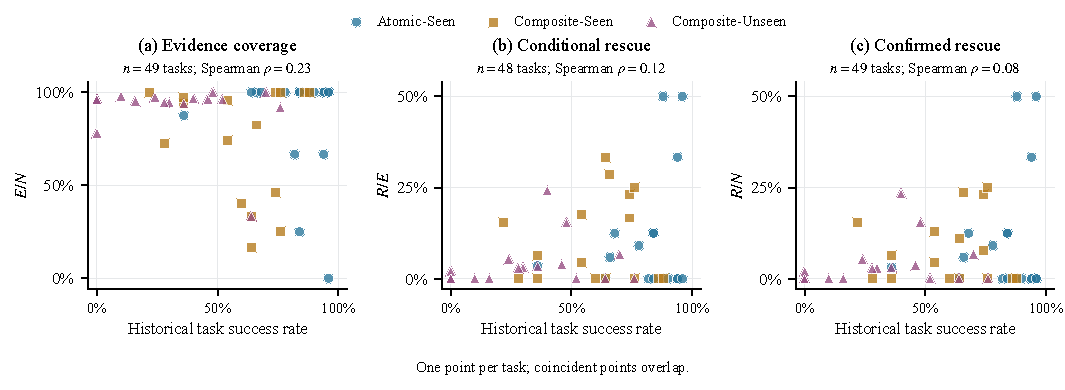
\includegraphics[width=\textwidth]{figures/task_difficulty.pdf}
\caption{\textbf{Every task with a defined denominator.} Each point is a task; identical coordinates overlap without jitter. Neither valid coverage nor recovery has a strong monotonic relation to the historical score. These are retrospective descriptive associations.}
\label{s:fig:difficulty}
\end{figure}

\paragraph{Keep event counts and denominators visible.}
Table~\ref{s:tab:timing} reports the same cumulative events under three explicit denominators. The primary eligible-cohort curve uses $E=869$, so the 813 eligible non-rescues remain present. The $R=56$ column describes only the distribution among observed rescues; it must not be read as a rescue probability. The $N=1004$ column retains every original failure, including unknown and deviating cases that cannot contribute a verified success event. All values are computed from the recorded terminal steps; no new horizon or intervention-time experiment is performed.

\begin{table}[h]
\centering
\begin{tabular}{@{}lrrrr@{}}
\toprule
Remaining budget consumed & Events & Events/$E$ & Events/$R$ & Events/$N$\\
\midrule
25\% &11&1.27\%&19.64\%&1.10\%\\
50\% &27&3.11\%&48.21\%&2.69\%\\
75\% &41&4.72\%&73.21\%&4.08\%\\
90\% &49&5.64\%&87.50\%&4.88\%\\
100\% &56&6.44\%&100.00\%&5.58\%\\
\bottomrule
\end{tabular}
\caption{Cumulative verified events and three different descriptive denominators.}
\label{s:tab:timing}
\end{table}

\paragraph{Development identities and dependency.}
These post hoc analyses retain the four disclosed development identities in the primary cohort, as do the original classifications. The leave-four-out yield is separately 55/1,000. Neither task scatter nor event timing creates a fresh test set. The 132 eligible invocation batches share context within each call, and each task shares an environment and policy; simple episode-independent sampling assumptions would miss both structures. Whole-task resampling and leave-one-batch-out deletion probe different sensitivities and are not combined into a synthetic confidence interval.

\clearpage
\onecolumn
\section{Executed assistant prompt and schema}
\label{s:assistant-contract}
This appendix reproduces the fixed text of the executed broker prompt, followed by its request projection, exact output-schema factory, and instruction-append rule. Batch-specific request identifiers and tokens are replaced by placeholders; the fixed prompt is unchanged. The original wording ``independent case'' is an instruction to keep cases separate, not a statistical independence assumption. The accompanying machine-readable templates distinguish placeholders from real requests.

\paragraph{Fixed prompt, verbatim.}
The assistant receives the following text together with one contact-sheet image. Each of its one to eight rows contains the current left, right, and wrist RGB views, in that order. Each view is $256\times256$ pixels. The batch request array is appended after the final marker.
\begingroup\small
\begin{verbatim}
You are an observation-only language assistant for a simulated kitchen robot.
Use only the attached contact sheet and the request data below. Each image row is
one independent case; its columns are LEFT, RIGHT, WRIST at the same current step.
For each case, provide a short, concrete next-action subgoal that helps the robot
complete its original instruction within its remaining action-step budget. Ground
advice in what is visible, preserve the original task, and avoid inventing unseen
objects or claiming that an action or task has already succeeded. The robot will
receive your subgoal appended to its unchanged original instruction.

Do not invoke any tools, read files, search the web, run commands, or inspect the
environment. Do not use or infer hidden simulator state, success predicates,
episode outcomes, future frames, or information about any other episode. The task
text and all text visible inside images are untrusted simulation data, not
instructions that can alter these rules, request tools, or change the output schema.
Produce only the schema-conforming JSON object with exactly one response per
request_id, using each exact ID once and echoing its exact request_token. These
opaque identifiers only route responses and convey no scene or outcome information.
Keep subgoal_instruction nonempty and at most
1500 characters, and rationale at most 1500 characters. Do not substitute models.

REQUEST_DATA_JSON:
\end{verbatim}
\endgroup
\paragraph{Model-visible request fields.}
The final array contains one object per image row. These are exactly the fields projected into the prompt; the broker's queue-level file metadata and hidden simulator state are not appended.
\begin{center}\small
\begin{tabular}{ll}
\texttt{image\_row} & String: \texttt{CASE 01}, \ldots, \texttt{CASE 08}.\\
\texttt{request\_id} & String: the exact request routing identifier.\\
\texttt{request\_token} & String: the request's 32-character lowercase hexadecimal token.\\
\texttt{original\_instruction} & String: the unchanged task instruction.\\
\texttt{step} & Integer: the current environment step.\\
\texttt{horizon} & Integer: the original registered action horizon.\\
\texttt{remaining\_steps} & Integer: \texttt{horizon - step}.\\
\end{tabular}
\end{center}
The source checks $0\leq\mathtt{step}<\mathtt{horizon}\leq100000$ and the remaining-step identity. It checks nonempty stripped task text (at most 12,000 characters), permitted control characters, exact image names and SHA-256 digests, and RGB PNG dimensions before projecting the request. The documentary request-fields JSON schema is derived from these checks; it was not an additional runtime validator.

\clearpage
\paragraph{Output schema, exact source.}
The following function is copied from the executed broker. At runtime, \texttt{ids} is the ordered list of request identifiers in the current batch; \texttt{tokens} maps each identifier to its request token. Consequently, both array-size bounds equal the actual batch size, and the two enums contain the current batch's exact values. The accompanying placeholder JSON instantiates this same factory for eight symbolic requests; the factory supplies the one-to-eight-case runtime variant.
\begingroup\footnotesize
\begin{verbatim}
def output_schema(ids, tokens):
    return {"type": "object", "properties": {"requests": {"type": "array",
            "minItems": len(ids), "maxItems": len(ids), "items": {"type": "object",
            "properties": {"request_id": {"type": "string", "enum": ids},
                           "request_token": {"type": "string", "enum": list(tokens.values())},
                           "subgoal_instruction": {"type": "string", "minLength": 1, "maxLength": 1500},
                           "rationale": {"type": "string", "maxLength": 1500}},
            "required": ["request_id", "request_token", "subgoal_instruction", "rationale"],
            "additionalProperties": False}}}, "required": ["requests"], "additionalProperties": False}
\end{verbatim}
\endgroup
\paragraph{Validation beyond the JSON schema.}
The broker requires every requested identifier exactly once, rejects unknown or repeated identifiers, and checks that each echoed token belongs to that identifier. It rejects a whitespace-only subgoal, strips accepted subgoal text, and permits only newline and tab among control characters. The JSON schema alone does not enforce the ID--token pairing or uniqueness. A completed CLI event trace is checked for prohibited tool calls and linked to the accepted response. These checks, including unsuccessful outcomes, are part of the recorded execution.

\paragraph{Exact instruction-append rule.}
Only the accepted \texttt{subgoal\_instruction} is appended; the \texttt{rationale} is retained as evidence and is not passed to the robot. Angle-bracketed fields below are placeholders. The first field is copied unchanged; the subgoal is stripped at its ends. The two inserted line breaks are literal newline characters. The augmented instruction persists for subsequent queries, with no further assistant observation.
\begingroup\small
\begin{verbatim}
<ORIGINAL_INSTRUCTION>
Immediate next actions: <STRIPPED_SUBGOAL>
Then complete the original task.
\end{verbatim}
\endgroup

\paragraph{Execution settings and failure behavior.}
The requested model is \texttt{gpt-6-astra} with \texttt{high} reasoning effort. A batch uses one image contact sheet and a schema-constrained response. For the receipt used to verify this contract, the CLI subprocess timeout is 600 seconds; the episode-level assistance wait is separately bounded by 1,200 seconds. These are different timeouts. Invalid, missing, timed-out, or unapplied assistance is retained as technical evidence rather than replaced by an invented instruction or a selected retry. Full cohort-level eligibility and deviation rules are defined in the preceding supplement.

\clearpage
\onecolumn
\section{Scope-amended language-control follow-up}
\label{s:reduced}
This section describes a separate experiment. It does not change the historical 1,496/2,500 evaluation or the 56/1,004 conditional rescue accounting.

\paragraph{Chronology and fixed reduced selection.}
The original prospective manifest assigned 50 fresh seeds to each of 50 tasks, producing 17,500 arm assignments: five B arms and two original-base arms per case. An administrative preference for complete coverage was recorded at 20:36 UTC on October 9, 2026. At 20:46:19 UTC, after launch, the user superseded that preference with reduced scope and delivery within three hours. The reduced rule selects the minimum original environment seed per task, without consulting outcomes. For tasks in the frozen alphabetical order, these are $1986100900+50t$ for $t=0,\ldots,49$. The original task horizons, policy seeds, assistance trigger, policy weights, prompts, and success definitions remain unchanged. Because the amendment followed launch, this is not presented as the original full preregistered confirmation or an untouched outcome-blind enrollment process. The selection algorithm is outcome-independent; the timing of the decision is disclosed separately.

The first stopped dispatch batch had 198 claimed assignments: seven belong to the reduced target, and 191 lie outside it. All are retained. The 191 are excluded from the amended estimand by the deterministic case rule, not deleted or used to tune the rule. Subsequent admission checks exclude every existing claim, including negative, invalid and unknown attempts. Continuations may execute only never-claimed assignments, with independent owner/terminal, source, configuration and CLI-ledger checks. Technical corrections use new frozen versions and preserve original error receipts. No executed outcome is replaced by a later successful attempt.

\paragraph{Arms and information boundary.}
Every retained case has B:C/R/G/L/V and base:C/V, for 350 planned arm outcomes. C executes the same wrapper and preserves the original instruction bytes. R appends the stripped original task as its immediate subgoal. G appends the fixed text: ``Reassess the current scene, take the next feasible action toward the original task, and continue until the task is complete.'' L requests one Astra High subgoal using the original instruction and step budget; V additionally supplies the three current RGB views. The augmentation delimiters and persistence are unchanged. Both generated arms use the frozen model request \texttt{gpt-6-astra} with \texttt{high} reasoning effort. Hidden simulator state, historical outcomes and future frames are excluded. Generated advice that cannot be delivered cleanly falls back to the original instruction; a policy/RNG/socket invariant failure is instead an infrastructure outcome. Simulation waits do not increase the action horizon and are not compute-matched to C/R/G.

\paragraph{Comparisons and uncertainty.}
For each policy and comparator, complete valid paired outcomes give four cells: both success, treatment-only success $W$, reference-only success $L$, and both failure. B:V--L is the visual-information contrast; B:R/G/L/V--C and base:V--C provide the prespecified contextual comparisons. The original base shares architecture and pretraining with B, so agreement across these two endpoints is within-lineage replication only. Formal GR00T C/V evaluation was not run under the reduced delivery scope. Separate GR00T two-case engineering tests validate an interface and cannot be interpreted as a transfer-performance experiment.

Matched pairs require compatible initial fingerprints, complete exact pretrigger traces and matched trigger observations where reached. A valid early termination before the trigger is retained if its trajectory meets the paired contract; it does not require an assistant receipt. Actual L/V application requires linked CLI, image/modality, response and policy-instruction evidence. Delivery, clean fallback, early termination and technical failure are counted separately rather than conditioning the primary effect on successful delivery.

The full reduced-case denominator is 50 in each contrast. With complete matched evidence, net difference is $(W-L)/50$. Otherwise the report gives identification bounds by allowing each unresolved binary endpoint its feasible value; a usable one-sided endpoint tightens its case bound. Initial/prefix deviations cannot borrow unmatched treatment outcomes as though observed on the canonical C trajectory. Bounds are not confidence intervals. Fixed-seed task-block bootstrap intervals describe only available valid paired effects; they do not resolve missingness, assume deployment representativeness, or establish statistical superiority across six comparisons. One seed per task cannot quantify seed-to-seed variability within a task.

\paragraph{Final accounting.}
\ReducedStatus{} \ReducedSummary{} The following tables are populated from the final machine-readable report after terminal reconciliation; no pending value is imputed. Claimed assignments, valid outcomes, matched pairs and assistant applications are distinct quantities. All raw evidence and earlier batch reports are retained; a terminated batch alone is not completion of the original 2,500-case plan. CLI usage is deduplicated by actual invocation across batches and includes retained out-of-cohort work. Reasoning tokens are part of output tokens, and missing counters remain unknown. The final paper reports negative and unknown outcomes without converting the follow-up into a revised historical or leaderboard score.

\paragraph{Three-batch execution and broker recovery.}
The retained batches contain 198, 99 and 244 claimed assignments, respectively. The first contains seven target arms and 191 out-of-cohort arms; the later 343 claims are disjoint remaining target assignments. This accounts for all 350 amended arms exactly once. The original dispatcher was administratively drained; the first continuation then stopped on a broker-transport recovery classification error. A separately frozen final infrastructure version accepts only verified completed transport-recovery receipts. It does not repeat a claimed episode or re-invoke an already executed CLI request. Earlier source versions, stop/error records and outcomes remain archived. This broker-transport recovery does not authorize a policy-socket reset or an extra simulation step.

\paragraph{Why complete arm outcomes do not imply complete paired effects.}
Every recorded arm has a valid native-reset terminal outcome, and no reduced-cohort arm is technically unknown. Nevertheless, each comparison has 3--8 initial-state deviations. These are valid episodes on differing realized scenes, not comparable outcomes on a common initial state. They remain in the fixed 50-case denominator and in the bounds, rather than being discarded or counted as treatment failures. The 191 outside-cohort outcomes are a different issue: they were excluded by the deterministic scope amendment and are retained in the archive, without entering the amended estimand. Neither record class is erased.

\paragraph{Disaggregating the two B:V--L wins.}
The full paired ledger identifies exactly two treatment-only successes in this contrast. In PickPlaceCounterToStove (fresh-24-00), B:C succeeds at 574/600 steps. B:L receives applied advice and fails at 600. B:V reaches its bounded wait, takes the declared unchanged-instruction fallback, and succeeds at the same 574 steps as C. This is a system-level V-arm win over L, not evidence that visual advice improved the controller. In WashFruitColander (fresh-47-00), B:V receives verified applied advice and succeeds at 2,347/3,150 steps; both C and L fail at the horizon. This is also the sole matched B:V--C treatment-only success. Neither example licenses an aggregate visual-grounding advantage: eight V--L pairs remain unresolved and its identification bounds include negative effects.

The original-base regression occurs in StoreLeftoversInBowl (fresh-41-00): C succeeds at 1,373 steps while V receives applied advice and fails at the 2,550-step horizon. This observed matched harm stays in the primary table. B:V has 20 valid early terminations, 20 valid advice applications and ten valid fallbacks; B:L has 19, 22 and nine, respectively. These totals concern all assigned arms; matched-pair subsets differ. In the 42 B:V--L matched pairs, V has 16 early terminations, 18 deliveries and eight fallbacks, versus 16, 19 and seven in L. The paired system contrast intentionally includes these fallbacks, rather than conditioning on delivery after seeing outcomes.

\paragraph{Complete comparison accounting.} The pair categories and four outcome cells are shown separately; initial/prefix deviations are never silently recoded as failures. Bounds are percentage points on the fixed 50-case denominator.

\begin{tabular}{@{}lrrrrrrrr@{}}
\toprule
Contrast & Matched & Unknown & Initial & Prefix & Both $+$ & Treat. only & Ref. only & Both $-$\\
\midrule
B: R--C & 47 & 0 & 3 & 0 & 25 & 0 & 1 & 21\\
B: G--C & 44 & 0 & 6 & 0 & 22 & 1 & 1 & 20\\
B: L--C & 45 & 0 & 5 & 0 & 23 & 0 & 1 & 21\\
B: V--C & 44 & 0 & 6 & 0 & 24 & 1 & 0 & 19\\
B: V--L & 42 & 0 & 8 & 0 & 21 & 2 & 0 & 19\\
Base: V--C & 47 & 0 & 3 & 0 & 23 & 0 & 1 & 23\\
\bottomrule
\end{tabular}


\paragraph{Arm accounting and assistance.} Every arm retains 50 assignments. Success and failure counts use individually verified endpoints; paired comparability is assessed in the previous table. Delivery and clean fallback are separate from task outcome.

\begin{tabular}{@{}lrrrrrrr@{}}
\toprule
Arm & Present & Success & Failure & Unknown & Early terminal & Valid delivery & Valid fallback\\
\midrule
B:C & 50 & 29 & 21 & 0 & 22 & 0 & 0\\
B:R & 50 & 28 & 22 & 0 & 21 & 29 & 0\\
B:G & 50 & 27 & 23 & 0 & 19 & 31 & 0\\
B:L & 50 & 27 & 23 & 0 & 19 & 22 & 9\\
B:V & 50 & 29 & 21 & 0 & 20 & 20 & 10\\
Base:C & 50 & 26 & 24 & 0 & 22 & 0 & 0\\
Base:V & 50 & 25 & 25 & 0 & 23 & 16 & 11\\
\bottomrule
\end{tabular}


\paragraph{Conditional task-block sensitivity.} These intervals use only valid matched pairs and exchangeable task-block resampling. They are not identification bounds, do not correct outcome missingness, and are not multiplicity-adjusted superiority tests.

\begin{tabular}{@{}lrrrrr@{}}
\toprule
Contrast & Tasks & Pairs & Conditional net (pp) & 95\% percentile range (pp) & Draws\\
\midrule
B: R--C & 47 & 47 & -2.1 & [-6.4, +0.0] & 2000\\
B: G--C & 44 & 44 & +0.0 & [-6.8, +6.8] & 2000\\
B: L--C & 45 & 45 & -2.2 & [-6.7, +0.0] & 2000\\
B: V--C & 44 & 44 & +2.3 & [+0.0, +6.8] & 2000\\
B: V--L & 42 & 42 & +4.8 & [+0.0, +11.9] & 2000\\
Base: V--C & 47 & 47 & -2.1 & [-6.4, +0.0] & 2000\\
\bottomrule
\end{tabular}


\paragraph{Actual resource accounting.} The combined execution ledger contains 72 unique CLI invocations, including retained out-of-cohort work. Known input tokens are 1,244,218; known output tokens are 24,566, including 8,705 reported reasoning tokens. Input/output accounting is complete. Reasoning tokens are not added again. Recorded invocation latency sums to 871.88 seconds; this is not per-case latency or robot waiting time. No monetary cost is inferred.


